\section{Theory}
The lock-in amplifier is a device, which can measure very small AC voltages in the
presence of noise. It uses the principle of phase sensitive detection. It produces a maximum DC output
when the signal to be measured is in phase with a
reference signal at the same frequency. The lock-in
amplifier using AD630 chip is low cost and for the
teaching purpose of phase sensitive detection. It has
limited frequency and input voltage ranges of about
frequency range 200 Hz to 2 kHz and input voltages
of few microvolts.

\subsection*{Theoretical Considerations}
Amplifiers typically operate with a bandwidth spanning several kilohertz, and they are subject to various sources of noise. One common type is flicker
noise, which is present in all electronic instruments
and has a power spectrum that inversely varies with
frequency. This noise becomes problematic primarily at very low frequencies. Another source of noise
originates from electromagnetic interference, such as
that produced by running motors, fluorescent lights,
and similar devices. This type of noise exhibits a
peak in its power spectrum at the specific frequency
of the interfering source, like the motor or mains frequency, and can be mitigated using electromagnetic
shielding.

A third significant source of noise is thermal noise,
which is thermodynamic in origin and unavoidable.
Its power spectrum extends across all frequencies,
earning it the name "white noise”. In a circuit with
a resistance R through which a current I flows,
the voltage across the resistance fluctuates randomly
around the average value $V_0 = IR$. The mean square
fluctuation of the voltage, denoted as $\left\langle(V - V_0)^2\right\rangle$,
is calculated over a long time period. If this noise
is measured over a bandwidth W, the mean square
voltage is given by:

\begin{align}
    \left\langle(V - V_0)^2\right\rangle = 4k_BTRW
\end{align}

where $k_B$ is the Boltzmann constant, and $T$ is the
temperature.

To minimize thermal noise, one can either reduce
the temperature $T$ or decrease the bandwidth $W$ of
the amplifier. When detecting very weak signals at
room temperature, it is often necessary to effectively
reduce the bandwidth to just a few Hertz, despite the
amplifier’s typical kilohertz range. This reduction is
achieved using a technique known as Phase Sensitive Detection.

Consider an AC sinusoidal signal, such as the current
through the primary coil of a mutual inductance or
a periodically modulated light signal. The resulting
effect, such as the induced emf in the secondary coil,
will have the same frequency as the cause but may
differ in phase. For example, the induced emf will be
$\pi/2$ out of phase with the current in the primary coil
but will share its frequency. This effect is often weak,
in the range of microvolts or nanovolts. Amplifying
this weak signal directly also amplifies noise, which
can overwhelm the signal, especially in an amplifier
with a wide frequency range. To overcome this noise
and enhance the weak signal, a reference signal in
phase with the cause is used. Thus we can write

\begin{align}
    V_\text{signal} &= V_0 \sin(\omega t+\phi)\\
    V_\text{ref} &= V_0 \sin(\omega t)
\end{align}

Let’s consider the magnitudes of the signal and reference voltage after amplification in our circuit. These
signals are then fed into the AD 630 chip, a phasesensitive detector. This chip contains two identical
amplifiers: a noninverting amplifier, where the output is in phase with the input, and an inverting amplifier, where the output is 180° out of phase with
the input.

A comparator within the chip operates a switch
based on the reference signal.
The comparator’s
rapid response time, combined with the high slew
rate and fast settling of the amplifiers, minimizes
switching distortion. When the reference signal is
positive (during $0 < t < T/2$), the comparator directs the weak signal $V\text{signal}$ to the noninverting amplifier, producing an output

\begin{align}
    V_\text{out} = \mu V_\text{signal}\text{, for } 0 < t < T/2
\end{align}

\begin{figure}
    \centering
    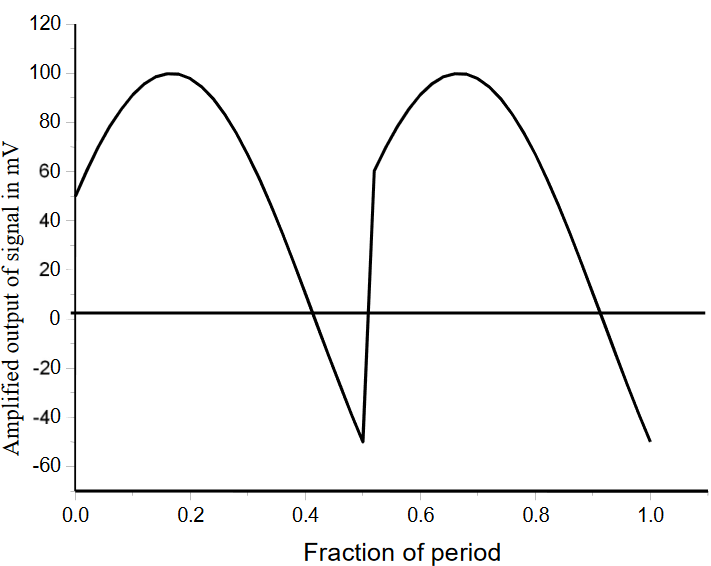
\includegraphics[width=.7\columnwidth]{images/f1.png}
    \caption{Amplified output $V_\text{out}$ when the reference signal is fed to the
    comparator.}
\end{figure}

\begin{figure}
    \centering
    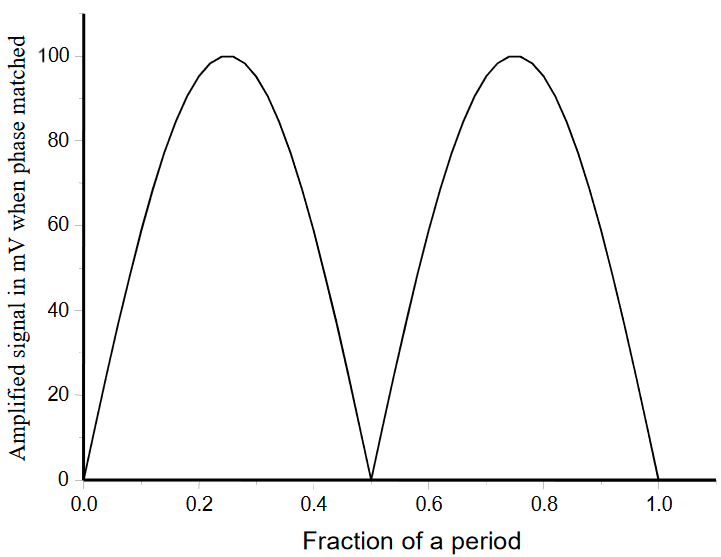
\includegraphics[width=.7\columnwidth]{images/f2.png}
    \caption{Amplified output signal when the reference signal is phase
    Shifted by $\phi$ and fed to AD630 chip}
\end{figure}

When the reference signal is negative (during
$T/2 < t < T$), the weak signal is routed to the inverting amplifier, resulting in an output:

\begin{align}
    V_\text{out} = -\mu V_\text{signal}\text{, for } T/2 < t < T
\end{align}

As shown in Figure 1, the output signal is positive
for most of the period, with a small negative portion.
This results in an output signal that includes both
an average DC component and an AC component at
frequencies $\omega$, 2$\omega$, and higher harmonics. By using a
filter that shunts the AC components to ground, the
DC output having a voltage $V_{dc}$ can be isolated.

The DC output can be calculated using the equation:

\begin{align}
    V_{dc} = \frac{1}{T}\int_0^{T/2}\mu V_0 \sin(\omega t + \phi)\,dt \nonumber\\
     - \frac{1}{T}\int_{T/2}^{T}\mu V_0 \sin(\omega t + \phi)\,dt
\end{align}

Simplifying this, and putting $\omega T = 2\pi$,

\begin{align}
    V_{dc} = \frac{4\mu V_0}{2\pi} \cos \phi
\end{align}

By introducing a phase-shift circuit for the reference signal before sending it to the comparator in
the AD 630, the output DC voltage will change as
the phase shift increases from zero. The DC voltage
peaks when the reference signal is phase-shifted by $\phi$,
aligning it in phase with the weak signal $V_\text{signal}$. At
this point, the output voltage resembles that shown
in Figure 2, and the average DC voltage $V_{dc}$ reaches
its maximum value of $2\mu V_0/\pi$. This technique is called
phase-sensitive detection, and the amplifier is known
as a lock-in amplifier because it locks the weak signal
in phase with the phase-shifted reference to maximize the DC output voltage.
By measuring the
phase shift needed to achieve this maximum output
on an oscilloscope, we can determine the phase difference between the effect and the cause.

If there is noise at a frequency $\omega'$ different from
the reference frequency $\omega$, using a large integration
time (much longer than the reference signal’s period)
significantly reduces its contribution to $V_{dc}$. Only
noise frequencies close to $\omega$, differing by $n/\tau$ (where
$n$ is a small number and $\tau$ is the integration time),
contribute to $V_{dc}$.
Therefore, the effective bandwidth of the lock-in amplifier is $n/\tau$. For an integration time of 1 second, the bandwidth $W$ is a few Hz,
effectively suppressing thermal and other noise.

\subsection*{Measurement of Mutual Inductance}
When two coils are placed side by side and an AC
current flows through one coil (the primary), an AC
voltage of the same frequency is induced in the other
coil (the secondary). If the primary current varies as

\begin{align}
    I = I_0 \sin(s\pi ft)
\end{align}

where f is the frequency in Hertz and the emf induced
in the secondary coil is given by

\begin{align}
    V = -M \frac{dI}{dt} = -2\pi MfI_0 \sin\left(2\pi ft + \frac{\pi}{2}\right)
\end{align}

From this, we observe that

\begin{itemize}
    \item The phase difference between the primary current and the induced emf is $\pi/2$.
    \item The induced emf is proportional to the amplitude $I_0$ of the primary current.
    \item The induced emf is also proportional to the frequency $f$.\\
\end{itemize}

We first plot the DC output of the Lock in Amplifier at different frequencies. Each plot is a straight
line. The intercept of the line increases with an increase in frequency. Now plot the slopes at different
frequencies along with the frequency. The slope of
this plot is given by

\begin{align}
    \beta = \frac{2 \pi M \mu}{R}
\end{align}

where $\mu$ is the amplification of Lock-in Amplifier and
$R$ is the resistance of the primary circuit. Knowing
$R$ and $\mu$ we can get M.

\subsection*{Measurement of Low Resistance}

Measurement of low resistance (resistance less than
an Ohm) with the DC technique would require a
high current. Also since the voltage developed across
the resistance will be small, it will be affected by
broadband noise when it is amplified.

If we plot the graph between $V_{dc}$ and $V_{ac}$ then the
slope is given by $\frac{dV_{dc}}{dV_{ac}}$ . Now,

\begin{align}
    dV_{ac} = R\,dI_{ac}
\end{align}

where $R$ is the total resistance in the primary circuit and $dI_{ac}$ is the change in the
current through the low resistance as the voltage changes by
$dV_{ac}$. The output $V_{dc}$ is proportional to the voltage $V_r$ across the low
resistance $r$. When the current through the low resistance is changed by $dI_{ac}$, the
voltage $V_r$ changes by $dV_r$,

\begin{align}
    dV_r &= r\,dI_{ac}\\
    \implies dV_{dc} = \mu dV_r &= \mu r\,dI_{ac} = \frac{\mu r}{R}dV_{ac}\\
    \implies \frac{dV_{dc}}{dV_{ac}} &= \frac{\mu r}{R}
\end{align}

% ======================================================================================
\section{Experimental Setup}

\subsection*{Apparatus}

\begin{enumerate}
    \item Lock-in amplifier
    \item Oscilloscope
    \item Breadboard and connecting wires
    \item Function Generator
    \item Test low resistance
    \item Resistances
    \item BNC cables
    \item Test mutual Induction Coil
    \item Digital Multimeter
\end{enumerate}